\subsection{Synchronous Fault-Tolerant OM(1) Systems}
\label{ssec:synchronous-om1}

\subsubsection{Informal Model}
Our first case study is is a system that implements one of the ``Oral Messages''
algorithms. These are synchronous, distributed, and fault-tolerant systems that
solve the Byzantine Generals Problem~\cite{Lamport-OM}. The family of systems
that implement $\OM{m}$ have different numbers of communicating nodes and
offer varying levels of fault tolerance. We've chosen to focus our attention
on systems that implement the specific algorithm $\OMH{1}$, ``Hybrid Oral
Messages with 1 Round''.  In this algorithm, $n$ nodes communicate in order to
reach agreement on a valid course of action (or equivalent information). This
is done in the presence of \emph{at most 1} faulty node, whose communications
and behavior are assumed to be completely unconstrained (``Byzantine''). The
difference between \OM(1) and \OMH(1) lies in the details of how certain types
of faulty messages are treated. \OMH(1) can be viewed as an extension of
\OM(1) which tolerates a broader set of fault patterns.

Figure~\ref{fig:om1} depicts the communication pattern for \OM{1} (and also
\OMH(1)). Each of the $n$ nodes in the system represents a (Byzantine)
General. In this formulation, the center node is the commanding general, while
the $n-1$ outer generals are the lieutenants. The algorithm starts with the
commanding general sending each lieutenant the same message $v$. Upon receipt
of the commander's message, each lieutenant in turn sends the message received
to each of the other lieutenants.  Once a lieutenant has received all $n-1$
expected messages, a majority vote is taken among the $n$ messages and the
lieutenant declares its output (course of action) to be whichever message is
in the majority.

\begin{figure}[ht]
\centering
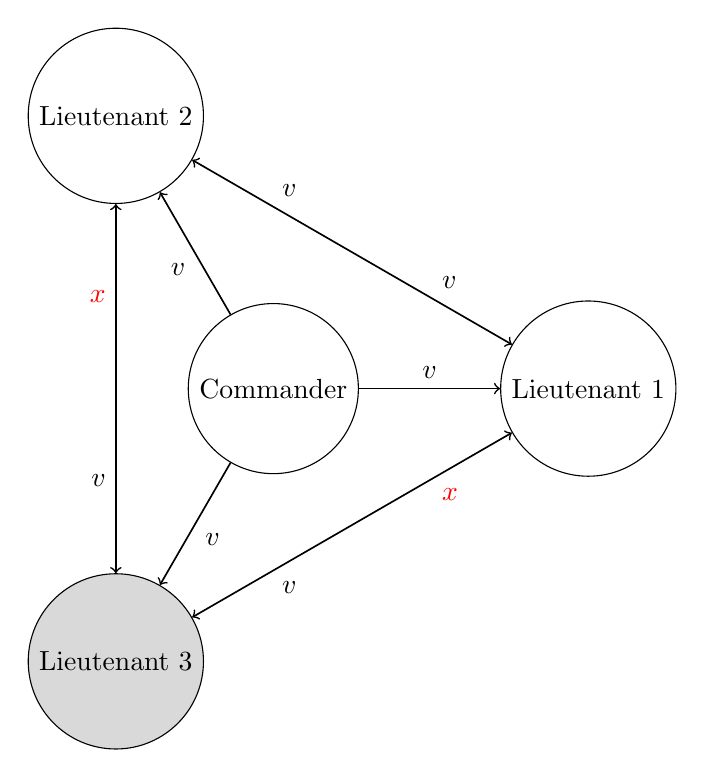
\begin{tikzpicture}[
ell/.style={x radius=1, y radius=0.5, draw, shape=circle},
arr/.style={semithick}]
\node[ell] (c)  at (0,0)   {Commander};
\node[ell] (l1) at (0:4)   {Lieutenant 1};
\node[ell] (l2) at (120:4) {Lieutenant 2};
\node[ell] (l3) [fill=gray!30] at (240:4) {Lieutenant 3};
%
\draw[->, arr] (c) -- node[auto] {$v$} (l1);
\draw[->, arr] (c) -- node[auto] {$v$} (l2);
\draw[->, arr] (c) -- node[auto] {$v$} (l3);
\draw[<->, arr] (l1) -- node[auto,swap,near start] {$v$}
                        node[auto,swap,near end] {$v$} (l2);
\draw[<->, arr] (l1) -- node[auto,near start,color=red] {$x$}
                        node[auto,near end] {$v$} (l3);
\draw[<->, arr] (l2) -- node[auto,swap,near start,color=red] {$x$}
                        node[auto,swap,near end] {$v$} (l3);
\end{tikzpicture}
\caption{\OMH{1} Four generals, one traitor}
\label{fig:om1}
\end{figure}

For a fault model we follow~\cite{Rushby-OM1} and assume that nodes are the
only source of faults. Moreover, node faults are assumed to be either
\emph{manifest}, \emph{symmetric}, or \emph{byzantine}. A fault is called manifest if
it is detectable by the non-faulty nodes; for example a node that sends to
another node a message that explicitly indicates there is a fault. On the
other hand, a fault is called symmetric if its presence is not necessarily
detectable as a fault to the other components; for example a node which sends
wrong messages, as opposed to invalid or missing messages.

Given a formal model of \OMH{1}, the standard target for verification is
\emph{validity} and \emph{agreement}. If we let $l_i$ denote the output for
lieutenant $i$ (where $1 \le i \le n-1$), then validity states:
%
\begin{equation}
    \forall \,i. \quad l_i = v
\end{equation}
%
whereas agreement states:
%
\begin{equation}
    \forall \,i, j. \quad l_i = l_j
\end{equation}
%
where $i,j$ range over the non-faulty nodes.

It is a classical result that \OM{1} can tolerate at most 1 (byzantine) faulty
node as long as there are at least 4 nodes in total. By adding additional
communication rounds, \OM{1} can be extended to an algorithm \OM{m} which
tolerates at most $m$ faults. On the other hand it is known that any system
which tolerates $m$ byzantine faults must involve at least $3m+1$ nodes.

In the results above there are several assumptions made regarding the
underlying computational platform which aren't obvious from the informal
description, but become so when one considers formally modelling it. To make
as many assumptions as possible explicit, we require:
\begin{enumerate}
    \item every message sent by a node is received successfully by the
        addressed node,
    \item when a node receives a message it may determine who sent it,
    \item each node can detect the absence of a message.
\end{enumerate}
These are the assumptions made by Lamport in his constructed solution for
$\OM{m}$ and the corresponding impossibility result (see
\cite{Lamport-OM}~\S2). It follows that a system implementing $\OM{1}$ must
transition synchronously. In particular, in an asynchronous system there is no
general method for detecting when a message is absent.

%% In Section~\ref{sssec:case-om1-sal} we present a formal model of $\OM{1}$ that
%% is the result of translating our ADSL specification to the transition system
%% language of SAL.

\subsubsection{ADSL Specification}

We now describe our implementation of Oral Messages in the ADSL. While we have specified
and verified the extension, \OMH(1) in the ADSL, we elide for simplicity the
differences between \OMH(1) and \OM(1) and just present \OM(1) here.

Our ADSL implementation of \OM(1) makes heavy use of the facilities of the
host language, Haskell. Indeed, the main part of the definition of the system
is given in just a few lines thanks to the use of parameterization.

\begin{figure}
\begin{lima}
om1 :: Atom ()
om1 = do
  -- setup channels for communication between source, relays, and receivers
  s2rs <- mapM newChannel ["s2r" ++ show i | i <- relaySet]
  r2rs <- mapM (mapM newChannel) [["r2r" ++ show i ++ show j | j <- recvSet]
                                                             | i <- relaySet]
  -- declare the set of vote variables that receivers will populate
  votes <- mapM msgVar ["vote" ++ show j | j <- recvSet]

  -- declare source node
  source (map fst s2rs)

  -- declare relay nodes
  forM_ relaySet 3 \idt ->
    relay ident (snd (s2rs !! idt))
                (map fst (r2rs !! idt))

  -- declare receiver nodes
  dones <- forM recvSet # \idt ->
    recv idt [snd ((r2rs !! i) !! idt) | i <- relaySet] (votes !! idt)

  -- state the "agreement" property
  let votesEqual (v,w) = value v ==. value w
  assert "agreement" # imply (and_ (map value dones))
                             (all_ votesEqual
                                   [(v,w) | v <- votes, w <- votes])

  -- state the "validity" property
  let voteGood v = value v ==. goodMsg
  assert "validity" # imply (and_ (map value dones)) (all_ voteGood votes)
\end{lima}
\caption{Setting up \OM(1)}
\label{fig:om1-setup}
\end{figure}

In this specification we refer to the Commander as the ``source'' and the
Lieutenants are unrolled into two sets: ``relays'' and ``receivers''. Here,
the source broadcasts to the relays which, in turn, broadcast to the
receivers which proceed with their vote. The code of Figure~\ref{fig:om1-setup} shows first channels being setup for communication, then
the source is declared by calling a function which we define shortly. The
relays and receivers are also declared by calling functions provided different
parameters. Note, the functions \y{forM} and \y{forM\_} are standard Haskell
constructs for defining iterations, i.e. ``for loops''.

For example, Figure~\ref{fig:om1-relay} shows the function definition for a
generic relay.

\begin{figure}
\begin{lima}
recv :: Int           -- ^ receiver id
     -> [ChanOutput]  -- ^ channels from relays
     -> V MsgType     -- ^ vote variable
     -> Atom (V Bool)
relay idt inC outCs = atom ("relay" ++ idt) # do
  -- declare local variables
  done <- bool "done" False
  msg  <- msgVar ("relay_msg" ++ idt)

  -- activation condition:
  --   we haven't stored a value yet and there is a message waiting
  --   on the channel 'inC'
  cond # isMissing msg &&. fullChannel inC

  -- behavior
  m <- readChannel inC
  msg  <== m
  done <== true
  forM_ outCs # \c -> writeChannel c m
\end{lima}
\caption{Function for declaring a generic relay}
\label{fig:om1-relay}
\end{figure}

The \y{relay} function takes an identifier, an incoming channel (for
receiving) and a list of channel outputs (for broadcasting). Recall that the
\y{cond} primitive acts as a guard on the atomic action to be taken in the
last 4 lines of the definition. In those last lines, the relay reads a message
from the incoming channel, stores it in a local variable, sets its \y{done}
flag, and then writes that message out on each of the outgoing channels it has.

The definition of \y{recv} is similar, except that each receiver possibly makes two
atomic actions through the declaration of two sub-atoms. The first sub-atom
listens for messages from the relays and fills a buffer as they arrive. The
second sub-atom is enabled only when the buffer is full and it computes a
majority vote on the buffer and stores the result in its \y{vote} variable
argument.

The majority vote computation is specified using the ``Fast Majority Vote''
algorithm due to Boyer and Moore \cite{mjrty}. This algorithm requires only a
single pass over the vote buffer. This is accomplished in our DSL using a
right fold operation as seen in Figure~\ref{fig:majority-vote}. A buffer value
and a counter are maintained during the pass. When the next element in the
buffer equals the currently maintained value, the counter is increased. If the
next element is different and the counter is zero, then the maintained value
is replaced, else the counter is decreased. In this way, at the end of the
pass, if there is a majority, it will be equal to the value maintained. It is worth
pointing out here that it is precisely this aspect, the level of detail in
implementing the majority vote, that sets our model of \OM(1) apart from
previous models.

\begin{figure}
\begin{lima}
computeVote :: [E MsgType] -> E MsgType
computeVote = fst . foldr iter (missingMsgValueE, 0)
  where
    iter x (y, c) = ( mux (x ==. y) onTrue1 onFalse1
                    , mux (x ==. y) onTrue2 onFalse2)
      where
        onTrue1       = y
        onTrue2       = c + 1
        onFalse1      = mux (c ==. 0) x y
        onFalse2      = mux (c ==. 0) 1 (c - 1)
\end{lima}
\caption{Fast Majority Vote in LIMA}
\label{fig:majority-vote}
\end{figure}

Finally, we have the system properties declared at the end of \y{om1} using
assertions. Both agreement and validity are predicated on the receivers being
done and the values in the list of vote variables.

\subsubsection{Generated Model}\label{sssec:om1-sally-model}

The formal model generated for \OM(1) by LIMA is quite large. Whereas the LIMA
specification file is only 5632 bytes, the Sally model LIMA generates for it
is 110,581 bytes. The generated model has 65 state variables, 12 input
variables, and 16 transitions in total. As an example of what the Sally model
looks like, consider the translation of the ``agreement'' property. Figure~\ref{fig:sally-query} shows the corresponding Sally query. The terms in the
query are rendered in $A$-normal form \cite{Sabry-Felleisen} to get maximum
benefit from sharing sub-terms.

\begin{figure}
\begin{sally}
(query
 om1_transition_system
 (let
  ((temp!0 true)
   (temp!1 om1!vote_2)
   (temp!2 om1!vote_1)
   (temp!3 (= temp!1 temp!2))
   (temp!4 om1!vote_0)
   (temp!5 (= temp!1 temp!4))
   (temp!6 (= temp!2 temp!1))
   (temp!7 (= temp!2 temp!4))
   (temp!8 (= temp!4 temp!1))
   (temp!9 (= temp!4 temp!2))
   (temp!10 (and temp!3 temp!5 temp!6 temp!7 temp!8 temp!9))
   (temp!11 (not temp!10))
   (temp!12 om1!recv_2!done)
   (temp!13 om1!recv_1!done)
   (temp!14 om1!recv_0!done)
   (temp!15 (and temp!11 temp!12 temp!13 temp!14))
   (temp!16 (not temp!15)))
  (not temp!15)))
\end{sally}
\caption{A Sally query rendered in $A$-normal form}
\label{fig:sally-query}
\end{figure}

Some verification of these models can be done automatically, without any
further work. For example, if we reduce \OM(1) system above so that it has
only 2 relays and 2 receivers, then the Sally model checker can automatically
verify that both agreement and validity hold in just over 11 minutes. With the
hybrid fault model assumption made, this is still a fairly non-trivial
verification and it is a highly non-trivial one for the model checker to
decide.
